% Created 2014-05-29 Thu 23:35
\documentclass[presentation]{beamer}
\usepackage[utf8]{inputenc}
\usepackage[T1]{fontenc}
\usepackage{fixltx2e}
\usepackage{graphicx}
\usepackage{longtable}
\usepackage{float}
\usepackage{wrapfig}
\usepackage{rotating}
\usepackage[normalem]{ulem}
\usepackage{amsmath}
\usepackage{textcomp}
\usepackage{marvosym}
\usepackage{wasysym}
\usepackage{amssymb}
\usepackage{hyperref}
\tolerance=1000
\usepackage{color}
\usepackage{listings}
\institute[Yale]{Yale School of Management}
\setbeameroption{show notes}
\usepackage{listings}
\usepackage{color}

\definecolor{mygreen}{rgb}{0,0.6,0}
\definecolor{mygray}{rgb}{0.5,0.5,0.5}
\definecolor{mymauve}{rgb}{0.58,0,0.82}

\lstset{ %
  numbers=left,                    % where to put the line-numbers; possible values are (none, left, right)
  numbersep=5pt,                   % how far the line-numbers are from the code
  numberstyle=\color{black}, % the style that is used for the line-numbers
  backgroundcolor=\color{white},   % choose the background color; you must add \usepackage{color} or \usepackage{xcolor}
  %basicstyle=\footnotesize,        % the size of the fonts that are used for the code
  basicstyle=\scriptsize,  
breakatwhitespace=true,         % sets if automatic breaks should only happen at whitespace
  breaklines=true,                 % sets automatic line breaking
  captionpos=b,                    % sets the caption-position to bottom
  commentstyle=\color{mygreen},    % comment style
  deletekeywords={...},            % if you want to delete keywords from the given language
  escapeinside={\%*}{*)},          % if you want to add LaTeX within your code
  extendedchars=true,              % lets you use non-ASCII characters; for 8-bits encodings only, does not work with UTF-8
  frame=single,                    % adds a frame around the code
  keepspaces=true,                 % keeps spaces in text, useful for keeping indentation of code (possibly needs columns=flexible)
  keywordstyle=\color{blue},       % keyword style
  %language=Octave,                 % the language of the code
  morekeywords={*,...},            % if you want to add more keywords to the set
  rulecolor=\color{black},         % if not set, the frame-color may be changed on line-breaks within not-black text (e.g. comments (green here))
  showspaces=false,                % show spaces everywhere adding particular underscores; it overrides 'showstringspaces'
  showstringspaces=false,          % underline spaces within strings only
  showtabs=false,                  % show tabs within strings adding particular underscores
  stepnumber=1,                    % the step between two line-numbers. If it's 1, each line will be numbered
  stringstyle=\color{mymauve},     % string literal style
  tabsize=2,                       % sets default tabsize to 2 spaces
  title=\lstname                   % show the filename of files included with \lstinputlisting; also try caption instead of title
}


\usepackage{attachfile2}
\usepackage{hyperref}
\setbeamertemplate{itemize/enumerate subbody begin}{\vspace{0.1cm}}
\setbeamertemplate{itemize/enumerate subbody end}{\vspace{0.1cm}}
\usetheme{Montpellier}
\usecolortheme{beaver}
\usefonttheme{professionalfonts}
\useinnertheme{rounded}
\useoutertheme{infolines}
\author{Robert Vesco}
\date{\today}
\title{Introduction to Python and Webscraping}
\hypersetup{
  pdfkeywords={},
  pdfsubject={},
  pdfcreator={Emacs 24.3.1 (Org mode 8.2.6)}}
\begin{document}

\maketitle

\section{Intro}
\label{sec-1}

\begin{frame}[label=sec-1-0-1]{Class Objectives}
\begin{itemize}
\item Programming is (can be) hard
\end{itemize}
\url{http://techcrunch.com/2014/05/24/dont-believe-anyone-who-tells-you-learning-to-code-is-easy/}

\begin{itemize}
\item Introduce basic python and webscraping
\item Provide skills \& knowledge not in online tutorials
\item Tools that can be used with any programming language
\item Provide some guidance for your personal projects
\end{itemize}
\end{frame}

\begin{frame}[label=sec-1-0-2]{Plan}
\begin{itemize}
\item Content
\begin{itemize}
\item Why Python?
\item Working From the Command Line
\item Python
\item Webscraping
\item Discuss sites YOU want to scrape
\item Development environments
\end{itemize}
\item Breaks 
\begin{itemize}
\item 10:30 (10 min)
\item 12:00 Lunch (30 min)
\item 1:30 (10 min)
\end{itemize}
\end{itemize}
\end{frame}

\section{Python Context}
\label{sec-2}

\begin{frame}[label=sec-2-0-1]{Opinionated  History of Programming Languages}
\begin{itemize}
\item Lisp
\item C, C++
\item Awk, Sed \& shell scripts
\item Practical Extraction and Reporting (perl)
\item S (R precursor)
\item Java
\item Ruby
\item R
\item Haskell
\item Clojure (Incanter)
\item Python
\item Julia
\end{itemize}
\end{frame}

\begin{frame}[label=sec-2-0-2]{Python and Stats}
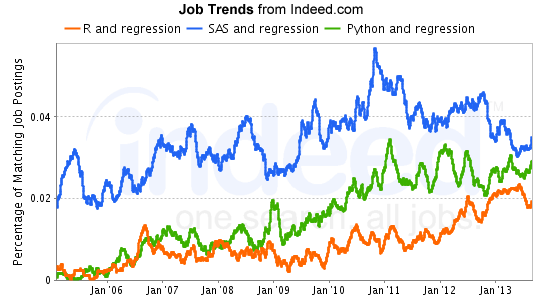
\includegraphics[width=.9\linewidth]{./images/lang_and_regression.png}
\end{frame}

\begin{frame}[label=sec-2-0-3]{Python and Journals}
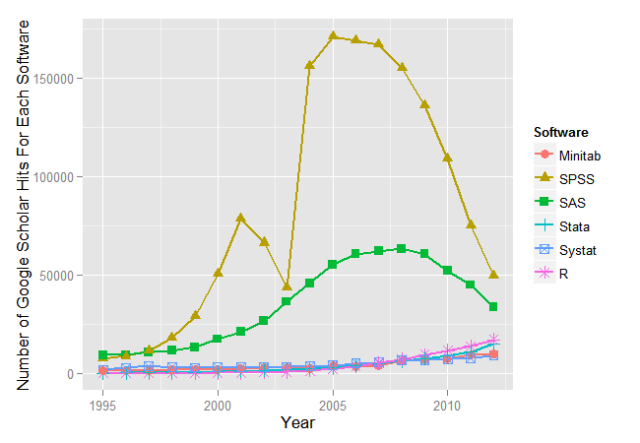
\includegraphics[width=.9\linewidth]{./images/lang_in_journals.png}
\end{frame}

\begin{frame}[label=sec-2-0-4]{Homogenization of Programming}
\url{http://www.talyarkoni.org/blog/2013/11/18/the-homogenization-of-scientific-computing-or-why-python-is-steadily-eating-other-languages-lunch/} 

\begin{itemize}
\item TLDR: One tool for many problems
\end{itemize}
\end{frame}

\begin{frame}[label=sec-2-0-5]{Python Considerations}
\begin{columns}
\begin{column}{0.4\textwidth}
\begin{block}{Support For}
\begin{itemize}
\item Readability \& Consistency (pythonic)
\item Fairly fast
\item Not Java
\item Used in biz ops \& domains
\end{itemize}
\end{block}
\end{column}

\begin{column}{0.4\textwidth}
\begin{block}{Support Against}
\begin{itemize}
\item Backward compatibility
\item Fragile package dependencies
\item Fragmentation
\item Complementary Assets for Science
\end{itemize}
\end{block}
\end{column}
\end{columns}
\end{frame}

\begin{frame}[label=sec-2-0-6]{The many faces and versions of Python}
\begin{itemize}
\item Cython (python to c to python)
\item IronPython (.net)
\item PyPy (JIT)
\item Jython (Java)
\item Ipython (scientific and interactive)
\end{itemize}
\end{frame}

\begin{frame}[label=sec-2-0-7]{Version 2 vs 3}
Python 3 is killing Python
\url{https://medium.com/@deliciousrobots/5d2ad703365d/} 

Python 3 can revive Python
\url{https://medium.com/p/2a7af4788b10}
\end{frame}

\begin{frame}[label=sec-2-0-8]{Interactive Python (IPYTHON)}
\begin{itemize}
\item Designed for interactive work \& scientists
\item Lots of useful features
\begin{itemize}
\item Tab completion
\item object?, object??
\item \%run scriptname
\item press up shows last command
\item \%who shows all variables
\item !cmd lets you run terminal commands
\end{itemize}
\item Terminal friendly
\end{itemize}
\end{frame}
\section{Terminals}
\label{sec-3}

\begin{frame}[label=sec-3-0-1]{Why Terminals and Command Line Programs?}
\begin{itemize}
\item Troubleshooting python programs
\item Managing programs and files (very important for webscraping)
\item Right tool for some jobs
\end{itemize}
\end{frame}

\begin{frame}[fragile,label=sec-3-0-2]{CD - Change Directory}
 \lstset{numbers=left,language=sh,label= ,caption= }
\begin{lstlisting}
pwd #your current path or %pwd 

mkdir test_dir #create directory

ls -laG #Show all files in directory

cd test_dir #folder = directory

cd ../../ #move up two directories

cd - #move back to last directory

cd #move to home directory

cd ~/test_dir #move to folder relative to home directory

touch test_dir/test_file.txt

rmdir test_dir #must be empty, so fails

rm -rf test_dir #-rf = recursive and force -- dangerous
\end{lstlisting}
\end{frame}


\begin{frame}[fragile,label=sec-3-0-3]{Open files in text editor}
 \begin{itemize}
\item Mac
\end{itemize}
\lstset{numbers=left,language=sh,label= ,caption= }
\begin{lstlisting}
open -t filename.ext #default editor for extension
open -a TextEdit filename.ext #forces textedit
#alias textedit='open -a TextEdit' For .bashrc
\end{lstlisting}
\begin{itemize}
\item Windows
\end{itemize}
\lstset{numbers=left,language=sh,label= ,caption= }
\begin{lstlisting}
notepad filename.txt
\end{lstlisting}
\begin{itemize}
\item Terminal Viewer (useful for super large files)
\end{itemize}
\lstset{numbers=left,language=sh,label= ,caption= }
\begin{lstlisting}
less -SN filename.txt
\end{lstlisting}
\end{frame}


\begin{frame}[fragile,label=sec-3-0-4]{Finding programs and scripts}
 \begin{itemize}
\item Depends on operating system
\end{itemize}

\lstset{numbers=left,language=sh,label= ,caption= }
\begin{lstlisting}
where python
whereis python
which python
\end{lstlisting}
\end{frame}


\begin{frame}[label=sec-3-0-5]{Sudo, Elevated Rights, Admin}
\begin{itemize}
\item Mac/Linux: sudo cmd file
\item Windows: runas /user:admin
\item Best to minimize programs running at elevated rights
\item Modifying system files usually require this.
\end{itemize}
\end{frame}


\begin{frame}[fragile,label=sec-3-0-6]{File Permissions}
 \lstset{numbers=left,language=sh,label= ,caption= }
\begin{lstlisting}
ls -laG #show all files and permissions
\end{lstlisting}

D = directory \\
4 = Read (r) \\
2 = Write (w) \\
1 = Execute(x) \\
777 = All rights for User, Group, Everyone <= BAD

\begin{itemize}
\item What is rwx-rw-r-- in numerical permissions?

\item Scripts will often need execution rights
\end{itemize}
\lstset{numbers=left,language=sh,label= ,caption= }
\begin{lstlisting}
chmod +x filename
\end{lstlisting}
\end{frame}

\begin{frame}[fragile,label=sec-3-0-7]{Simple Scripts}
 \lstset{numbers=left,language=sh,label= ,caption= }
\begin{lstlisting}
echo "print 'hello world'" > test.py

ls -laG #look at the file 

python test.py 

echo "#\!/usr/bin/python \n print 'hello world'" > test.py
./test.py
\end{lstlisting}

\begin{itemize}
\item How can we make the second way work?
\end{itemize}

\note{Notes:
}
\end{frame}



\begin{frame}[label=sec-3-0-8]{Find}
\url{http://www.tecmint.com/35-practical-examples-of-linux-find-command/}
\end{frame}


\begin{frame}[label=sec-3-0-9]{Shells vs Terminals}
\begin{itemize}
\item Shells are programs (like python) that help you interact computer.
\begin{itemize}
\item csh (c shell, mostly seen on older servers)
\item bash (most common)
\item zsh (most convenient)
\end{itemize}
\item Terminals are wrappers around shells (iterm2 for macs)
\item .bashrc, .cshrc, .zshrc are configuration files for shells
\end{itemize}
\end{frame}


\begin{frame}[fragile,label=sec-3-0-10]{Paths}
 \begin{itemize}
\item One of the biggest causes of angst
\item Exists at system and user levels
\item Order matters; read first > read second
\end{itemize}
\lstset{numbers=left,language=sh,label= ,caption= }
\begin{lstlisting}
#in bash, zsh 

#in windows (dos)
path %path%;C:\Python #temp
# see control panel > environment variables for permanent
\end{lstlisting}
\begin{itemize}
\item Macs/linux
\end{itemize}
\lstset{numbers=left,language=sh,label= ,caption= }
\begin{lstlisting}
/etc/paths #admin levels for mac
/etc/environment #admin
~/.bashrc #user level for mac/linux
export PATH="$PATH:/usr/local/bin/python"
PATH=$PATH:/my/new/path #temporary
\end{lstlisting}
\end{frame}


\section{Python}
\label{sec-4}

\begin{frame}[fragile,label=sec-4-0-1]{Anaconda and Spydyer}
 \begin{itemize}
\item Anaconda is a pre-packaged python distribution for scientists
\item Spyder is an IDE (Integrated Development Environment)
\item Open a terminal or click spyder
\end{itemize}

\lstset{numbers=left,language=sh,label= ,caption= }
\begin{lstlisting}
anaconda/bin/spyder
\end{lstlisting}

\begin{itemize}
\item Open terminal within spyder
\end{itemize}
\end{frame}


\subsection{Basics}
\label{sec-4-1}

\begin{frame}[label=sec-4-1-1]{Programming Concepts}
\begin{itemize}
\item Types (int, strings)
\item Data Structures
\item Variables
\item Flow structures
\item Function, Objects and Modules
\item Scripting and Programs
\end{itemize}
\end{frame}


\begin{frame}[fragile,label=sec-4-1-2]{Hello World}
 \begin{block}{Version 2 - Print Statement}
\lstset{numbers=left,language=Python,label= ,caption= }
\begin{lstlisting}
print "hello world"
\end{lstlisting}
\end{block}

\begin{block}{Version 3 - Print Function}
\lstset{numbers=left,language=Python,label= ,caption= }
\begin{lstlisting}
print("hello world")
\end{lstlisting}
hello world
\end{block}

\note{Note
\begin{itemize}
\item stuff and stuff
\end{itemize}}
\end{frame}


\begin{frame}[fragile,label=sec-4-1-3]{Comments in Python}
 \lstset{numbers=left,language=Python,label= ,caption= }
\begin{lstlisting}
# This is a single line comment
print "stuff" # This is also a comment

'''
Multiline comments 
Are surround by triple-quoted strings
'''
\end{lstlisting}

\note{Notes:
\begin{itemize}
\item stuff and stuff2
\end{itemize}}
\end{frame}




\begin{frame}[fragile,label=sec-4-1-4]{Basic Types}
 \begin{itemize}
\item Numeric: int, float, long, complex
\item Sequence: str, unicode, list, tuple, bytearray, buffer, xrange
\end{itemize}
\lstset{numbers=left,language=Python,label= ,caption= }
\begin{lstlisting}
var1 = "test strings"
var2 = 3      
type(var1) 
type(var2)
var3 = str(3) # conversion is possible, sometimes
type(var3)
\end{lstlisting}

\lstset{numbers=left,language=Python,label= ,caption= }
\begin{lstlisting}
<type 'str'>
<type 'int'>
<type 'str'>
\end{lstlisting}
\end{frame}


\begin{frame}[label=sec-4-1-5]{Data Structures}
\begin{itemize}
\item Often considered "types" or "compound types"
\item Base python has
\begin{itemize}
\item lists = ['apples',44, 'peaches']
\item tuples = read-only lists = ('apples',44,'peaches')
\item dictionaries = key:value pairs = \{'firstname':'tom','lastname':'selleck'\}
\end{itemize}
\end{itemize}
\end{frame}


\begin{frame}[fragile,label=sec-4-1-6]{Lists: Slicing}
 \begin{itemize}
\item lists are flexible. They can be nested, shrunk, combined \ldots{}
\item Indexed starting with 0
\item Limitation: searching for elements when you don't know index \#
\end{itemize}

\lstset{numbers=left,language=Python,label= ,caption= }
\begin{lstlisting}
ls = [1,"a",2,"b", 1]
ls[0]
ls[0:2]
ls[:]
ls[1:]
ls[1:4:2] #last element in step. Easy way to get odd
\end{lstlisting}

\lstset{numbers=left,language=Python,label= ,caption= }
\begin{lstlisting}
1
[1, 'a']
[1, 'a', 2, 'b', 1]
['a', 2, 'b', 1]
['a', 'b']
\end{lstlisting}
\end{frame}


\begin{frame}[fragile,label=sec-4-1-7]{Lists: Adding and Removing Elements}
 \lstset{numbers=left,language=Python,label= ,caption= }
\begin{lstlisting}
ls # pre
ls.append("add to end")
ls.insert(1,"after second element")
ls.insert(-1, "after second to last")
ls.remove('a') # by value, not index
ls # post
ls.index('b')
ls.count(1)
\end{lstlisting}

\lstset{numbers=left,language=Python,label= ,caption= }
\begin{lstlisting}
[1, 'a', 2, 'b', 1]
>>> >>> >>> >>> [1, 'after second element', 2, 'b', 1, 'after second to last', 'add to end']
3
2
\end{lstlisting}
\end{frame}


\begin{frame}[fragile,label=sec-4-1-8]{Lists: Whole List Operations}
 \lstset{numbers=left,language=Python,label= ,caption= }
\begin{lstlisting}
# Concatenate two lists
ls.extend(["newlist added to old"])
ls.sort()
ls
ls.reverse()
ls
\end{lstlisting}

\lstset{numbers=left,language=Python,label= ,caption= }
\begin{lstlisting}
[1, 1, 2, 'add to end', 'after second element', 'after second to last', 'b', 'newlist added to old']
['newlist added to old', 'b', 'after second to last', 'after second element', 'add to end', 2, 1, 1]
\end{lstlisting}
\end{frame}


\begin{frame}[fragile,label=sec-4-1-9]{Lists: List Comprehensions}
 \begin{itemize}
\item Functions on list elements, like loops
\item Not recommended for complex scenarios
\end{itemize}

\lstset{numbers=left,language=Python,label= ,caption= }
\begin{lstlisting}
ls2 = [str(x) for x in ls]
ls2
## nested loop, + = concat for strings
[[x+y for x in ls2] for y in ls2]
\end{lstlisting}

\lstset{numbers=left,language=Python,label= ,caption= }
\begin{lstlisting}
['1', 'a', '2', 'b', '1']
[['11', 'a1', '21', 'b1', '11'], ['1a', 'aa', '2a', 'ba', '1a'], ['12', 'a2', '22', 'b2', '12'], ['1b', 'ab', '2b', 'bb', '1b'], ['11', 'a1', '21', 'b1', '11']]
\end{lstlisting}
\end{frame}


\begin{frame}[fragile,label=sec-4-1-10]{Sets}
 \begin{itemize}
\item Set are like lists, but must contain unique data and can't be nested
\item Allows operations such a union and intersections
\end{itemize}

\lstset{numbers=left,language=Python,label= ,caption= }
\begin{lstlisting}
ls_dupes = [1,2,3,4,4,3]
st = set(ls_dupes)
print st
st2 = {1,2,3,5}
print st | st2 # union
print st & st2 # intersection
lss = list(st & st2) # convert back
\end{lstlisting}

\lstset{numbers=left,language=Python,label= ,caption= }
\begin{lstlisting}
>>> set([1, 2, 3, 4])
>>> set([1, 2, 3, 4, 5])
set([1, 2, 3])
>>> <type 'list'>
\end{lstlisting}
\end{frame}


\begin{frame}[fragile,label=sec-4-1-11]{Tuples}
 \begin{itemize}
\item Tuples are like lists, but they are immutable
\item Memory efficient because python knows how much memory to allocate
\end{itemize}
\lstset{numbers=left,language=Python,label= ,caption= }
\begin{lstlisting}
tp = () # empty tuple
tp1 = (1,) #tuple with one element (comma required)
tp2 = (1,2,3)
tp
tp1
tp2
tp2[2] #slicing uses [] not ()
\end{lstlisting}

\lstset{numbers=left,language=Python,label= ,caption= }
\begin{lstlisting}
()
(1,)
(1, 2, 3)
3
\end{lstlisting}
\end{frame}


\begin{frame}[fragile,label=sec-4-1-12]{Dictionaries}
 \begin{itemize}
\item Represented by key:value pairs. Know as hashes, maps, associative collections
\item Key can be numbers or strings, but must be unique.
\item Value can be mutable or not, can be combined with tuples
\item Useful when you need a fast lookup based on custom key.
\end{itemize}

\lstset{numbers=left,language=Python,label= ,caption= }
\begin{lstlisting}
dct = {'first':1, 'second':2, 'third':3}
dct['second']
del(dct['third'])
dct.keys()
dct.values()
\end{lstlisting}

\lstset{numbers=left,language=Python,label= ,caption= }
\begin{lstlisting}
2
['second', 'first']
[2, 1]
\end{lstlisting}
\end{frame}


\begin{frame}[label=sec-4-1-13]{Operators}
\end{frame}


\begin{frame}[label=sec-4-1-14]{Control structures}
\end{frame}


\begin{frame}[fragile,label=sec-4-1-15]{Strings}
 \begin{block}{Strings vs Numbers}
\lstset{numbers=left,language=Python,label= ,caption= }
\begin{lstlisting}
string = "123456"
number = 123456 
string is number
int(string) is number # different "objects"
int(string)==number # testing equality of value
\end{lstlisting}

\lstset{numbers=left,language=Python,label= ,caption= }
\begin{lstlisting}
False
False
True
\end{lstlisting}
\end{block}


\begin{block}{Strings vs lists of strings}
\lstset{numbers=left,language=Python,label= ,caption= }
\begin{lstlisting}
a = [string]
b = [string]
a == b # compares equality
a is b # compares whether objects
\end{lstlisting}

\lstset{numbers=left,language=Python,label= ,caption= }
\begin{lstlisting}
>>> True
False
\end{lstlisting}
\end{block}
\end{frame}

\begin{frame}[fragile,label=sec-4-1-16]{Objects, Methods and Functions}
 \begin{itemize}
\item Methods are function that operate on objects
\item Object: dog Method: eat
\item Functions
\end{itemize}
\url{http://stackoverflow.com/questions/8108688/in-python-when-should-i-use-a-function-instead-of-a-method}


\lstset{numbers=left,language=Python,label= ,caption= }
\begin{lstlisting}
var1.capitalize() # method on object
len(var1) # also method, but functional looking
\end{lstlisting}

\lstset{numbers=left,language=Python,label= ,caption= }
\begin{lstlisting}
'Test strings'
12
\end{lstlisting}
\end{frame}


\begin{frame}[label=sec-4-1-17]{Modules}
\end{frame}

\begin{frame}[label=sec-4-1-18]{Dates}
\end{frame}

\begin{frame}[fragile,label=sec-4-1-19]{Functions}
 \begin{itemize}
\item parameter order matters, unless name=paramater
\item anonymous functions use lambda keyword
\item return statements without value return nothing
\item Variables within function have local scope
\end{itemize}

\lstset{numbers=left,language=Python,label= ,caption= }
\begin{lstlisting}
def printnum( x, y ):
    """This passes a parameter to the print statement"""
    print x, y
    return

printnum(y=3, x="printing this:")
printnum("positional ordering matter if not named", 4)
\end{lstlisting}

\lstset{numbers=left,language=Python,label= ,caption= }
\begin{lstlisting}
printing this: 3
positional ordering matter is not named 4
\end{lstlisting}
\end{frame}


\begin{frame}[label=sec-4-1-20]{Files I/O}
\end{frame}

\begin{frame}[fragile,label=sec-4-1-21]{CSV files - Basic}
 \lstset{numbers=left,language=sh,label= ,caption= }
\begin{lstlisting}
echo -e "header1, header2\n1,2\n3,4" > test.csv
\end{lstlisting}
\lstset{numbers=left,language=Python,label= ,caption= }
\begin{lstlisting}
import csv
fl = list(csv.reader(open("test.csv")))
header, values = fl[0], fl[1:]
header
values
fl
\end{lstlisting}

\lstset{numbers=left,language=Python,label= ,caption= }
\begin{lstlisting}
['head1', 'head2']
[['1', '2'], ['3', '4']]
[['head1', 'head2'], ['1', '2'], ['3', '4']]
\end{lstlisting}
\end{frame}

\begin{frame}[fragile,label=sec-4-1-22]{CSV files - Custom}
 \lstset{numbers=left,language=Python,label= ,caption= }
\begin{lstlisting}
class customcsv(csv.Dialect):
    lineterminator = '\n'
    delimiter = ','
    quoting = csv.QUOTE_NONE

fl.csv = csv.reader("test.csv", dialect=customcsv)
fl.csv
\end{lstlisting}
\end{frame}

\begin{frame}[fragile,label=sec-4-1-23]{CSV files - Pandas - read$_{\text{csv}}$}
 \lstset{numbers=left,language=Python,label= ,caption= }
\begin{lstlisting}
import pandas as pd
# header=none if not in file
# or read_table + sep(delimeter)
fldf = pd.read_csv("test.csv")
type(fldf) #type is different
fldf
\end{lstlisting}

\lstset{numbers=left,language=Python,label= ,caption= }
\begin{lstlisting}
<class 'pandas.core.frame.DataFrame'>
     head1  head2
0      1      2
1      3      4

[2 rows x 2 columns]
\end{lstlisting}
\end{frame}

\begin{frame}[label=sec-4-1-24]{CSV files - Pandas - More Options}
\begin{itemize}
\item nrow=5 => read 5 rows
\item na\(\textunderscore\)rep='NULL' => set null to NULL else empty
\item index=FALSE => no indices in output
\item cols=['header1','header2'] => specify columns
\item For all options:
\end{itemize}
\url{http://pandas.pydata.org/pandas-docs/version/0.13.1/generated/pandas.io.parsers.read_csv.html}
\end{frame}

\begin{frame}[fragile,label=sec-4-1-25]{CSV files - Pandas - to\(\_\)csv}
 \begin{itemize}
\item Many of the same options as read$_{\text{csv}}$
\end{itemize}
\url{http://pandas.pydata.org/pandas-docs/version/0.13.1/generated/pandas.DataFrame.to_csv.html}
\lstset{numbers=left,language=Python,label= ,caption= }
\begin{lstlisting}
import os #to see directory contents
fldf
fldf.to_csv("files/test_out.csv")
os.listdir('files')
\end{lstlisting}

\lstset{numbers=left,language=Python,label= ,caption= }
\begin{lstlisting}
head1  head2
0      1      2
1      3      4

[2 rows x 2 columns]
>>> ['test_out.csv']
\end{lstlisting}
\end{frame}


\begin{frame}[fragile,label=sec-4-1-26]{Getting Help}
 \begin{itemize}
\item help(function) gets you the "docstring"
\end{itemize}
\lstset{numbers=left,language=Python,label= ,caption= }
\begin{lstlisting}
help(len)
\end{lstlisting}

\lstset{numbers=left,language=Python,label= ,caption= }
\begin{lstlisting}
Help on built-in function len in module __builtin__:

len(...)
    len(object) -> integer

    Return the number of items of a sequence or mapping.
\end{lstlisting}
\end{frame}


\subsection{Advanced}
\label{sec-4-2}

\begin{frame}[label=sec-4-2-1]{Regular Expression}
\end{frame}

\begin{frame}[label=sec-4-2-2]{Expressions}
\end{frame}

\begin{frame}[label=sec-4-2-3]{Classes/Objects}
\end{frame}

\begin{frame}[label=sec-4-2-4]{Common Packages}
\begin{block}{Scientific}
\begin{itemize}
\item Numpy: N-dimensional arrays, C integration, linear algebra
\item SciPy: Numerical integration, optimization, depends on Numpy
\item Matplotlib: 2d plotting
\item Pandas: Approximates R/Stata, data cleaning, dataframes
\item Statsmodels: For statistical models
\end{itemize}
\end{block}
\begin{block}{Webscraping}
\begin{itemize}
\item BeautifulSoup
\end{itemize}
\end{block}
\end{frame}


\section{Webscraping}
\label{sec-5}

\subsection{Firefox/HTML}
\label{sec-5-1}

\begin{frame}[label=sec-5-1-1]{HTML/XML/JSON}
\begin{itemize}
\item HTML is an implementation of XML (a meta language)
\item JavaScript Object Notation (JSON) is replacing xml for speed and readability (api)
\end{itemize}
\end{frame}

\begin{frame}[label=sec-5-1-2]{Firebug}
\begin{itemize}
\item Firebug is tool that allow you to inspect the elements of a webpage
\end{itemize}
directly. 
\end{frame}


\subsection{XML}
\label{sec-5-2}

\begin{frame}[fragile,label=sec-5-2-1]{XPATH SQL for HTML/XML}
 \begin{itemize}
\item Xpath is a language that allows you to select "nodes" from xml
\item Note: xpath 2.0 not implemented in all cases though many examples online
\item Xpath 1.0 Tutorial
\end{itemize}
\begin{verbatim}
http://www.zvon.org/comp/r/tut-XPath_1.html#Pages~List_of_XPaths
\end{verbatim}
\begin{itemize}
\item Full reference
\end{itemize}
\url{http://www.w3.org/TR/xpath/} 
\end{frame}




\begin{frame}[fragile,shrink=1,label=sec-5-2-2]{XML - Loading}

 \lstset{numbers=left,language=Python,label= ,caption= }
\begin{lstlisting}
xml = """
    <root>
        <name type="superhero">Batman</name>
            <sidekick>Batty</sidekick>
        <contact type="email">riseup@batman.com</contact>
        <contact type="phone">555-1212</contact>
    </root>
            """

from lxml import objectify
root = objectify.fromstring(xml) #use parse from file

print root.tag
print root.text
print root.attrib

print root.name.tag
print root.name.text
print root.name.attrib

for con in root.contact:
    print con.text
    print con.attrib
\end{lstlisting}
\textattachfile[color =  0.5 0.5 0.5]{pdfxml.txt}{view source}
\end{frame}


\subsection{JSON}
\label{sec-5-3}

\begin{frame}[fragile,label=sec-5-3-1]{JSON - Loading}
 \lstset{numbers=left,language=Python,label= ,caption= }
\begin{lstlisting}
jsn = """
    {"name":"batman",
     "hobbies": ["fast cars", "fast planes", "spending money"],
    "buddy":"robin",
    "enemies": [{"name":"The Joker"},
                {"name":"The People of Gotham"}]
                }
"""
import json
#NOTE: loads for strings, load for files
rslt = json.loads(jsn) #put this into a form for python
print rslt
jsn_again = json.dumps(rslt) #back to json
\end{lstlisting}

\lstset{numbers=left,language=Python,label= ,caption= }
\begin{lstlisting}
{u'buddy': u'robin', u'enemies': [{u'name': u'The Joker'}, {u'name': u'The People of Gotham'}], u'name': u'batman', u'hobbies': [u'fast cars', u'fast planes', u'spending money']}
\end{lstlisting}
\end{frame}


\begin{frame}[fragile,label=sec-5-3-2]{JSON - Converting to DataFrames}
 \lstset{numbers=left,language=Python,label= ,caption= }
\begin{lstlisting}
enemies = pd.DataFrame(rslt['enemies'], columns=['name'])
enemies
\end{lstlisting}

\lstset{numbers=left,language=Python,label= ,caption= }
\begin{lstlisting}
	      name
0             The Joker
1             The People of Gotham

[2 rows x 1 columns]
\end{lstlisting}
\end{frame}


\begin{frame}[fragile,label=sec-5-3-3]{JSON - Converting to DataFrames}
 \lstset{numbers=left,language=Python,label= ,caption= }
\begin{lstlisting}
enemies = pd.DataFrame(rslt['enemies'], columns=['name'])
enemies
\end{lstlisting}

\lstset{numbers=left,language=Python,label= ,caption= }
\begin{lstlisting}
	      name
0             The Joker
1  The People of Gotham

[2 rows x 1 columns]
\end{lstlisting}
\end{frame}


\begin{frame}[fragile,shrink=20,label=sec-5-3-4]{JSON - Example}

 \lstset{numbers=left,language=Python,label= ,caption= }
\begin{lstlisting}
import json
import urllib2
import pprint import pprint
import pandas as pd

prefix="http://maps.googleapis.com/maps/api/geocode/json?address="
suffix="&sensor=false"
address="165%20Whitney%20Avenue,%20New%20Haven,%20CT"
url = prefix+address+suffix
j = urllib2.urlopen(url)
js = json.load(j)
type(js) #if in doubt, check type

#pprint(js) 

#notice nested list, so use index to get into it
rstadd = js['results'][0]['address_components']

for rs in rstadd:
    print rs['short_name'], rs['types']

import pandas as pd
pd.DataFrame(rstadd)
\end{lstlisting}
\textattachfile[color =  0.5 0.5 0.5]{pdfjson.txt}{view source}
\end{frame}


\begin{frame}[label=sec-5-3-5]{Regular Expressions (Regex)}
\begin{itemize}
\item Regex came from perl, used to find text patterns
\item To fragile for webscraping, but important complement
\end{itemize}
\end{frame}


\section{Development}
\label{sec-6}

\subsection{Paths}
\label{sec-6-1}

stuff

\subsection{Other}
\label{sec-6-2}

Stuff



\begin{frame}[label=sec-7-0-1]{Git}
\url{http://wildlyinaccurate.com/a-hackers-guide-to-git}
\end{frame}

\subsection{Python}
\label{sec-7-1}
\begin{frame}[label=sec-7-1-1]{Operators}
\end{frame}

\begin{frame}[label=sec-7-1-2]{Setting Up Your Development Environment}
\end{frame}



\begin{frame}[label=sec-8-0-1]{Top Aligned Blocks}
\begin{columns}
\begin{column}{0.5\textwidth}
\begin{block}{Code}
Cool
Lots
of Stuf

To talk

about
\end{block}
\end{column}

\begin{column}{0.5\textwidth}
\begin{block}{Result}
pretty nice!
\end{block}
\end{column}
\end{columns}
\end{frame}


\subsection{Inline math}
\label{sec-8-1}


\begin{frame}[label=sec-8-1-1]{Beamer: Animated Bullets}
\begin{itemize}[<+->]
\item Trouble Shooting
\item A framework for thinking about programming
\end{itemize}
\end{frame}


\begin{frame}[label=sec-8-1-2]{Beamer Columns}
\begin{columns}
\begin{column}{0.5\textwidth}
\end{column}
\end{columns}
\begin{block}{Stuff}
\begin{itemize}
\item Truth is ephemeral
\end{itemize}
\end{block}


\begin{columns}
\begin{column}{0.5\textwidth}
\begin{itemize}
\item What is right?
\item What is Wrong?
\end{itemize}
\end{column}
\end{columns}
\end{frame}



\begin{frame}[fragile,label=sec-9-0-1]{setting python paths}
 \begin{verbatim}
:Setting environment variables (like PYTHONPATH)
:Create an emacs-lisp code block that looks like this:

:#+BEGIN_SRC emacs-lisp
:(setenv "PYTHONPATH" "/Users/neilsen/Development/obswatch-trunk/common/python")
:#+END_SRC
:Execute it, and it changes the environment accordingly.
:Note that you can also append to environment variables like this:

:#+BEGIN_SRC emacs-lisp
:(setenv "PYTHONPATH" (concat (getenv "PYTHONPATH") ":" (getenv "DQSTATS_DIR")))
:#+END_SRC
:#+END_SRC
\end{verbatim}
\end{frame}



\begin{frame}[fragile,label=sec-9-0-2]{How to use virtualenv \& pip}
 \lstset{numbers=left,language=sh,label= ,caption= }
\begin{lstlisting}
## run this on the command line
## assuming you are in your projects folder, create a new folder
mkdir projects1 

cd projects1

## now create your virtualenv environment
## this will create a folder called "env". 
## this will house a local version of python. 
virtualenv env 

## IMPORTANT. 
## Now you need to activate your environment. 
source env/bin/activate

## now you will be using a local version of python instead of your
## system's python

## to deactivate, simply type
deactivate
\end{lstlisting}
\end{frame}

\begin{frame}[label=sec-9-0-3]{How to Share Ipython Notebooks}
\end{frame}
\begin{frame}[label=sec-9-0-4]{How to share your vagrant box}
\end{frame}
\begin{frame}[fragile,label=sec-9-0-5]{Testing Python Output}
 \lstset{numbers=left,language=Python,label= ,caption= }
\begin{lstlisting}
a = ('b', 200)
b = ('x', 10)
c = ('q', -42)
return (a, b, c)
\end{lstlisting}
\end{frame}

\begin{frame}[fragile,label=sec-9-0-6]{Python Output}
 \lstset{numbers=left,language=Python,label= ,caption= }
\begin{lstlisting}
a = ('b', 200)
b = ('x', 10)
c = ('q', -42)
return (a, b, c)
\end{lstlisting}

By removing the :exports both, you can export just the code and not the output. By replaceing it with :exports results, you can export the output without the source. 
\end{frame}

\begin{frame}[fragile,shrink=1,label=sec-9-0-7]{Using pip once virtualenv is activated}

 \lstset{numbers=left,language=sh,label= ,caption= }
\begin{lstlisting}
## again, these should be run on the command line. 
## first, let's activate your virtual environment, if you haven't 
## already
source env/bin/activate

## first, let's inspect what command are available in pip
pip help

## from this, we see that there are a number of commands we will 
## find useful
pip list # this shows what programs are already installed
pip search numpy # this searches for packages named "numpy"
pip install numpy # this installs the numpy package. 

## if you have many packages you want to install, you can 
## create a requirements list
## this will create a file with a list of modules to install
## you can use your editor of choice to install this. 
echo "numpy\nbeautifulsoup" > requirements.txt

## this will install all the packages in the text file. 
## NOTE: you can specify the versions of module too. Sometimes
## this is important. 
pip install -r requirements.txt

## now let's confirm that they installed correctly
pip list 

## now if you are done with virtualenv remember to deactivate it
deactivate
\end{lstlisting}
\end{frame}



\section{CheatSheets}
\label{sec-10}

\subsection{Python}
\label{sec-10-1}

\begin{frame}[label=sec-10-1-1]{Operators}
\tiny
\begin{center}
\begin{tabular}{|c|p{2in}|l|}
Operator & Description & Example\\
+ & Addition - Adds values on either side of the operator & a + b will give 30\\
- & Subtraction - Subtracts right hand operand from left hand operand & a - b will give -10\\
* & Multiplication - Multiplies values on either side of the operator & a * b will give 200\\
\% & Modulus - Divides left hand operand by right hand operand and returns remainder & b \% a will give 0\\
** & Exponent - Performs exponential (power) calculation on operators & a**b will give 10 to the power 20\\
// & Floor Division - The division of operands where the result is the quotient in which the digits after the decimal point are removed. & 9//2 is equal to 4 and 9.0//2.0 is equal to 4.0\\
\end{tabular}
\end{center}
\end{frame}
% Emacs 24.3.1 (Org mode 8.2.6)
\end{document}